% 	This template is  MIT licensed.

% 	Basic file to demonstrate the usage of this LaTeX template.
% 	You can build your own paper/thesis on top of this file.
% 	Simply adjust the document class and all metadata and start working.
%
\documentclass[
	language=english, % set to english or german
	type=master, % set to bachelor, master or seminar
]{isthesis}

\usepackage[utf8]{vietnam}

% custom package
\usepackage{eurosym}
\usepackage{makecell}
\usepackage{hyperref}
\usepackage[utf8]{inputenc}
\usepackage{tabto} 
\usepackage{longtable}
% \usepackage{multirow}
% \usepackage{floatrow}

% Graphics rendering using TikZ
% See: https://en.wikibooks.org/wiki/LaTeX/PGF/TikZ
\usepackage{tikz}
\usepackage{xcolor}
\definecolor{light-gray}{gray}{0.95}
\newcommand{\code}[1]{\colorbox{light-gray}{\texttt{#1}}}
% Include required TikZ libraries here, some exemplary libraries are pre-included
\usetikzlibrary{calc}
\usetikzlibrary{matrix}
\usetikzlibrary{positioning}
\usetikzlibrary{shapes.geometric}

%Add your library here
\addbibresource{library.bib}

% Import acronyms
% \newacronym[longplural={<long plural>}, shortplural={<short plural>}]{<label>}{<short>}{<long>}
% 	label = is the unique identifier and sort key for the acronym, can be the same as <short>
%	short = is the abbreviation or acronym
%	short plural (optional) = is the plural of the abbreviation or acronym
%	long = is the long form of the acronym, this will appear in the list of abbreviations
%	long plural (optional) = is the long plural form of the abbreviation or acronym

\newacronym[shortplural={KMUen}, longplural={Kleine und Mittlere Unternehmen}]{kmu}{KMU}{Kleines und Mittleres Unternehmen}
\newacronym{CD}{CD}{Corporate Design}
\newacronym{SQL}{SQL}{Structured Query Language}
\newacronym{FAU}{FAU}{Khoa Toán cơ tin}
\newacronym{BPM}{BPM}{Business Process Management}
\newacronym{npm}{NPM}{Node Package Manager}
\newacronym{diss}{DISS}{Digital Industrial Service System}

% Import symbols
% Syntax: <Symbol> <Label> <Name>
% The symbols are sorted by their labels
\addsymboltolist{$\Pi$}{Pi}{Projection}
\addsymboltolist{$\Join$}{Join}{Natural Join}
\addsymboltolist{$\sigma$}{Selection}{Selection}


% Import custom commands
% If you want to define custom commands, please do so here

% Import custom code block
% define listing code
\definecolor{codegreen}{rgb}{0,0.6,0}
\definecolor{codegray}{rgb}{0.5,0.5,0.5}
\definecolor{codepurple}{rgb}{0.58,0,0.82}
\definecolor{backcolour}{rgb}{0.95,0.95,0.92}

\lstdefinestyle{code}{
    backgroundcolor=\color{backcolour},   
    commentstyle=\color{codegreen},
    keywordstyle=\color{magenta},
    numberstyle=\tiny\color{codegray},
    stringstyle=\color{codepurple},
    basicstyle=\ttfamily\footnotesize,
    breakatwhitespace=false,         
    breaklines=true,                 
    captionpos=b,                    
    keepspaces=true,                 
    numbers=left,
    firstnumber=1,
    stepnumber=1,                    
    numbersep=5pt,                  
    showspaces=false,                
    showstringspaces=false,
    showtabs=false,                  
    tabsize=2,
    framesep=10pt,
    xleftmargin=10pt,
    xrightmargin=10pt,
    framexleftmargin=16pt,
    framextopmargin=2pt,
    framexbottommargin=2pt, 
    frame=tb, framerule=0pt,
}

\lstdefinestyle{algo}{
    backgroundcolor=\color{backcolour},   
    commentstyle=\color{codegreen},
    keywordstyle=\color{magenta},
    numberstyle=\tiny\color{codegray},
    stringstyle=\color{codepurple},
    basicstyle=\ttfamily\footnotesize\small\linespread{0.8},
    breakatwhitespace=false,         
    breaklines=true,                 
    captionpos=b,                    
    keepspaces=true,                 
    numbers=none,
    firstnumber=1,
    stepnumber=1,                    
    numbersep=5pt,                  
    showspaces=false,                
    showstringspaces=false,
    showtabs=false,                  
    tabsize=2,
    framesep=10pt,
    xleftmargin=10pt,
    xrightmargin=10pt,
    framexleftmargin=16pt,
    framextopmargin=2pt,
    framexbottommargin=2pt, 
    frame=tb, framerule=0pt,
    mathescape=true
}

\lstset{style=code}

% Document meta information
\isthesis{
    title={TIỂU LUẬN},
    sub-title={Một số vấn đề về đồ hoạ máy tính \\
    Giám sát hệ thống micro-services và vấn đề logging},
    author-name={Nguyễn Mạnh Linh, Nguyễn Đức Thịnh}, 
    % Separate multiple authors with commas
    % author-email={linhnguyen.code@gmail.com},
    % author-matriculation={MATRICULATION NUMBER},
    % author-phone={+49 XXXXXXXXX}, % Use international numbers format
    % author-address={STREET},
    % author-zip={ZIP},
    % author-city={CITY},
    principal-supervisor={TS. Nguyễn Thị Bích Thuỷ}, % This must be a professor
    % associate-supervisor={SUPERVISOR}, % This is your main supervisor, i.e., a post doc or doctoral student
    tutor-supervisor={}, % If required, define an additional supervisor resp. tutor here
    group-institute={Đại học Khoa học Tự nhiên},
    % group={Image Data Exploration and Analysis (IDEA) Lab},
    % studies={M.Sc. International Information Systems}, %your field of studies, i.e. Wirtschaftsinformatik or International Information Systems
    %
    %associate-group={}, % When the thesis is done in cooperation with another chair, add it here
    %associate-group-institute={}, % add cooperating institute or university here
    seminar={SEMINAR}, % The title of your seminar
    submission-date={2023-01-10}, % The date you handed in your document: Format yyyy-mm-dd
    primary-logo={assets/hus.png}, % Uses the FAU logo by default
    %primary-logo-height={}, % Uses 16mm as default height
    %secondary-logo={}, % Logo of the secondary institution (cooperating chair/university), USES Faculty logo by default
    %secondary-logo-height={} % Uses 16mm as default height
}


\begin{document}
    % Title page
    \newcounter{savepage}
    \maketitle

	% Quote
    % You can put an optional quote page in front of your content
    %   \quotepage[author={Arthur C. Clarke}]{
    %   	        Any sufficiently advanced technology is indistinguishable from magic.
    %   }
    
    % Table of contents
    \tableofcontents

    \begin{abstract}
    Ngoài việc lập trình thì vận hành và giám sát là khâu quan trọng trong vòng đời của một sản phẩn công nghệ (phần mềm). Vận hành một sản phẩm không hề dễ dàng hơn việc tạo ra nó. Khi một phần mềm được triển khai thực tế, lập trình viên cũng như người quản trị hệ thống luôn cần nắm rõ \textit{sức khoẻ} của sản phẩm ví dụ như phần mềm đang tiêu tốn bao nhiêu tài nguyên của máy tính, phần mềm xử lý yêu cầu nhanh hay chậm, hay có bao nhiêu lỗi xảy ra trong khung giờ... Những thông số hay độ đo này là thước đo để biết được sản phẩm có đủ tốt hoặc quan trọng hơn là cảnh báo sớm cho người làm phần mềm về những nguy cơ có thể xảy ra. Bài báo cáo này giới thiệu một loạt các kĩ thuật, độ đo, cách kết hợp những công cụ và việc vận dụng khéo léo giữa bản thân phần mềm (ghi log) và các công cụ đó. Trực quan hoá dữ liệu được sử dụng một cách triệt để nhằm tạo một cái nhìn từ tổng quan đến chi tiết giúp cho người vận hành hệ thống cũng như lập trình viên luôn giữ được phần mềm của mình trong tầm kiểm soát.
\end{abstract} 

    % \begin{abstract}
	%     % Add your abstract here:
        
	% 	% \lipsum[1]
	% \end{abstract}

    % List of figures (if you have figures)
    % \listoffigures

    % List of tables (if you have tables)
    % \listoftables
    
    % List of listings (if you have listings)
	% \lstlistoflistings

    % List of abbreviations (if you use acronyms)
    %\listofabbreviations

    % List of symbols (if you use symbols)
    %\listofsymbols
	
	% Abstract
	%
	% Comment out this part, if you don't require an abstract

	
	% storing the last pagenumber
    \setcounter{savepage}{\value{page}}
    
    
    % Content
    \begin{content}
        % Add your content files:
        \chapter{Giới thiệu}
\begin{figure}[H] % places figure environment here   
  \centering % Centers Graphic
  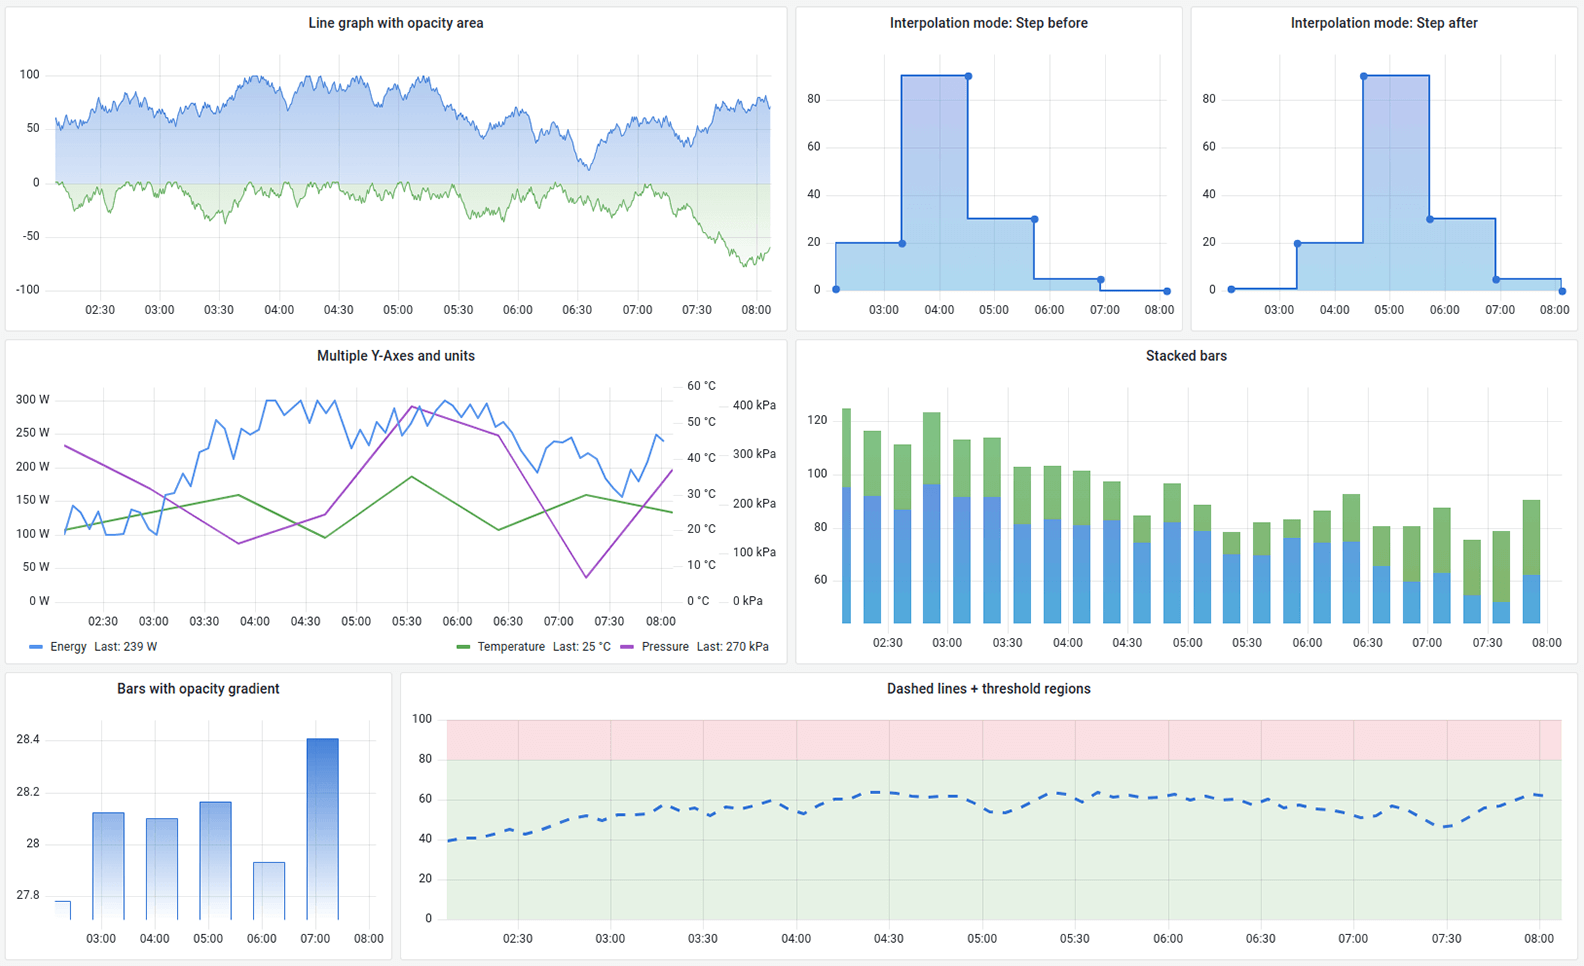
\includegraphics[width=0.8\textwidth]{figures/time_series_light_theme_sized.png} 
  \caption{Biểu đồ dữ liệu hướng thời gian} % Creates caption underneath graph
  \label{fig:fig_01}
\end{figure}

        \chapter{Hệ thống giám sát với Grafana}
\section{Giới thiệu Grafana}
Grafana là một nền tảng mã nguồn mở hỗ trợ mạnh mẽ cho việc theo dõi và đánh giá các số liệu thu thập được. Vì vậy, Grafana có thể được ứng dụng rộng rãi trong nhiều lĩnh vực khác nhau chứ không chỉ riêng công nghệ thông tin. Bất kì lĩnh vực nào có thể thu thập được dữ liệu theo dòng thời gian đều có thể tối ưu trực quan hóa trên Grafana.

Đối với việc quản trị vận hành phần mềm, Grafana là công cụ hỗ trợ mạnh mẽ việc trực quan hóa các chỉ số (ví dụ như cpu, ram, dish, network, iops, session,…) và nhật ký hoạt động được thu thập từ ứng dụng. Nó có thể kết nối được với nhiều nguồn dữ liệu khác nhau như Prometheus, InfluxDB, ElasticSearch và các công cụ cơ sở dữ liệu quan hệ truyền thống. Nhờ vậy mà ta có thể truy vấn, trực quan hóa, cảnh báo và tìm hiểu dữ liệu bất kể chúng được lưu trữ ở đâu, từ đó tạo ra những hệ thống giám sát sinh động, linh hoạt, dễ dàng nắm bắt thông tin và kiểm soát trạng thái của ứng dụng.
\begin{figure}[H] % places figure environment here   
    \centering % Centers Graphic
    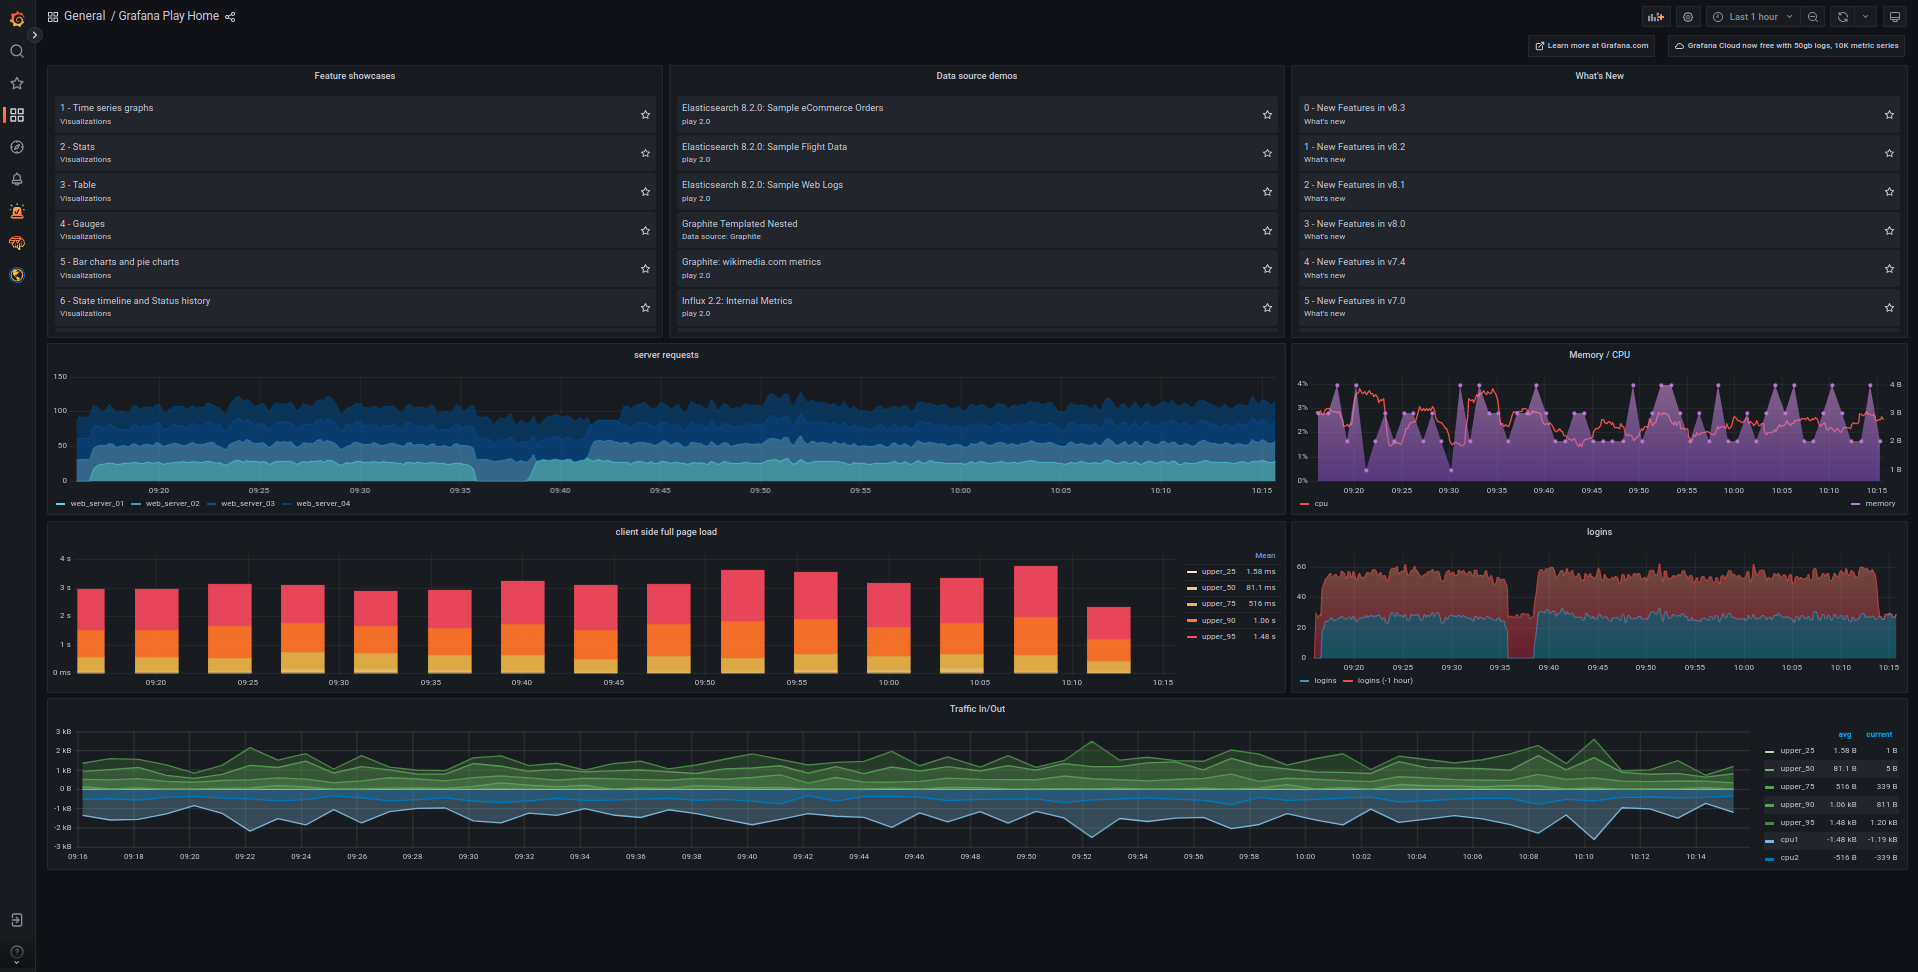
\includegraphics[width=1\textwidth]{figures/fig_01.png} 
    \caption{Một dashboard demo trên trang chủ của Grafana} % Creates caption underneath graph
    \label{fig:fig_01}
\end{figure}
Hình 2.1 thể hiện ví dụ về một dashboard được xây dựng với Grafana. Biểu đồ trên cùng bên trái thể hiện lượng requests tới một website nào đó trong khoảng thời gian một giờ gần nhất. Không chỉ thể hiện tổng lượng request, ta còn có thể quan sát thấy thông lượng tới từng node từ web\_server\_01 đến web\_server\_04 thông qua lớp phủ màu. Ngoài ra khi giữ chuột vào một thời điểm nhất định, biểu đồ cũng cho biết số lượng request cụ thể vào từng node vào thời điểm đó. Biểu đồ trên cùng bên phải thể hiện tài nguyên Memory và CPU được sử dụng của ứng dụng. Các biểu đồ tiếp theo lần lượt đưa ra các chỉ số khác cần theo dõi của ứng dụng.

\section{Case study}

        \chapter{Quản lý, giám sát và logging}
\section{Giới thiệu ELK-stack}
ELK Stack là từ viết tắt được sử dụng để mô tả bộ dịch vụ bao gồm 3 dự án phổ biến: Elasticsearch, Logstash và Kibana. Thường được gọi là Elasticsearch, ELK Stack mang tới khả năng tổng hợp log từ tất cả các hệ thống và ứng dụng của bạn, phân tích những log này, hiển thị dữ liệu để giám sát ứng dụng và cơ sở hạ tầng, khắc phục sự cố nhanh hơn, phân tích bảo mật, v.v. Không quan trọng webserver sử dụng NGINX, Apache hay MSServer, không quan trọng log đến từ ứng dụng, database, cache server... chúng đều có thể được xử lý bởi ELK!

\begin{figure}[H] % places figure environment here   
    \centering % Centers Graphic
    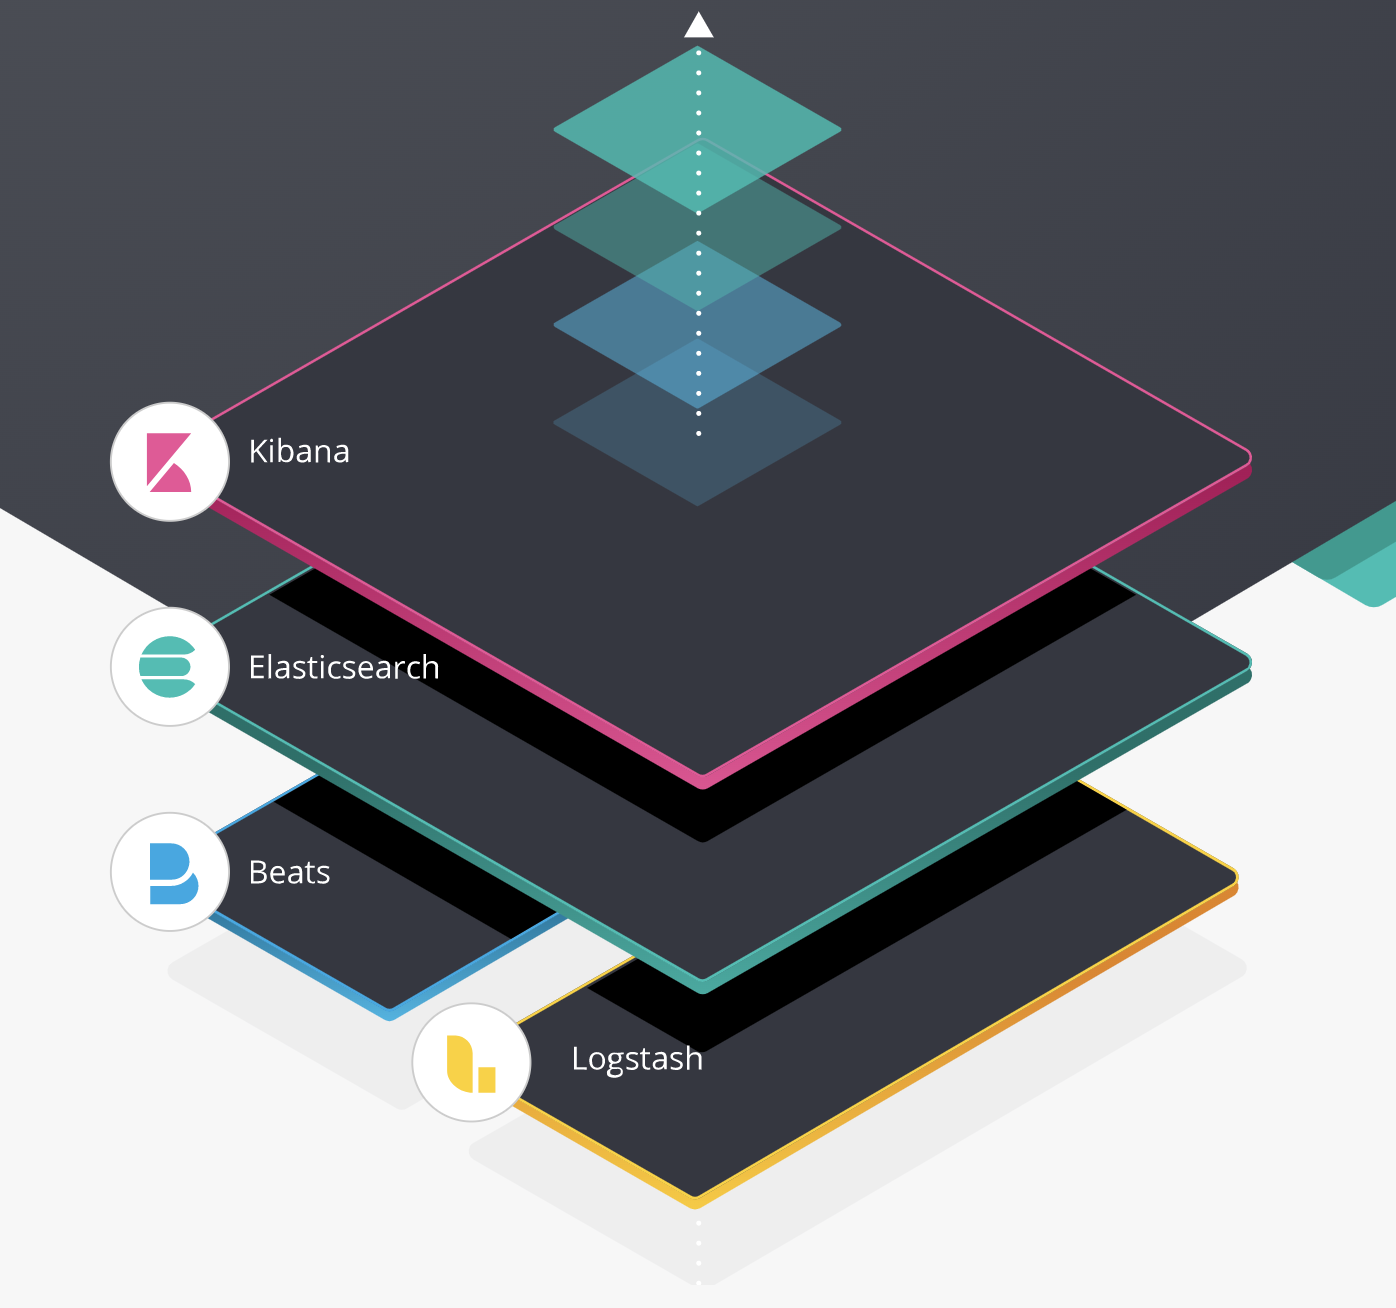
\includegraphics[width=0.8\textwidth]{figures/elk_02.png} 
    \caption{ELK stack} % Creates caption underneath graph
    \label{fig:elk_02}
\end{figure}

\begin{itemize}
    \item \textit{E = Elasticsearch}: Elasticsearch là công cụ tìm kiếm và phân tích phân tán được xây dựng trên Apache Lucene. Khả năng hỗ trợ đa dạng ngôn ngữ, hiệu suất cao và JSON doccument phi cấu trúc khiến Elasticsearch trở thành một lựa chọn lý tưởng cho nhiều trường hợp sử dụng tìm kiếm và phân tích log khác nhau.
    \item \textit{L = Logstash}: Logstash là một công cụ thu nạp dữ liệu nguồn mở cho phép thu thập dữ liệu từ các nguồn khác nhau, chuyển đổi dữ liệu và gửi dữ liệu tới điểm đích. Với các bộ lọc được tạo sẵn và hỗ trợ hơn 200 phần bổ trợ, Logstash cho phép người dùng dễ dàng thu nạp bất kỳ dữ liệu đến từ nguồn hay thuộc loại dữ liệu nào.
    \item \textit{K = Kibana}: Kibana là một công cụ hiển thị trực quan và khám phá dữ liệu dành cho hoạt động đánh giá log và sự kiện. Kibana cung cấp các biểu đồ tương tác dễ sử dụng, các bộ lọc được tạo sẵn cũng như hỗ trợ không gian địa lý. 
\end{itemize}

\begin{figure}[H] % places figure environment here   
    \centering % Centers Graphic
    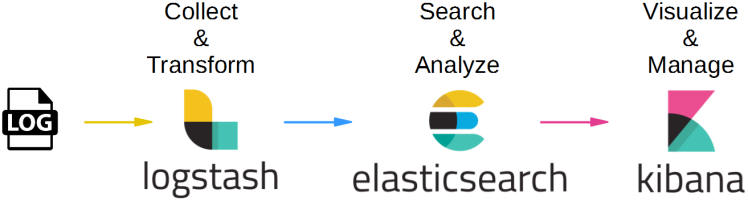
\includegraphics[width=0.6\textwidth]{figures/elk_01.png} 
    \caption{ELK stack với log ứng dụng} % Creates caption underneath graph
    \label{fig:elk_01}
\end{figure}
Nói một cách đơn giản thì Logstash là nơi tiếp nhận dữ liệu từ nhiều nguồn sau đó có thể biến đổi hoặc lọc bớt dữ liệu và ghi vào Elasticsearch. Elasticsearch vừa là nơi lưu trữ vừa là công cụ có khả năng tìm kiếm và phân tích. Kibana là công cụ trực quan hoá dữ liệu từ Elasticsearch, ngoài ra nó cũng cung cấp giao diện đơn giản để thực hiện truy vấn, phân tích với Elasticsearch dễ dàng hơn.
\section{Case study}
        \chapter{Kết luận}

Do mô hình đề xuất khá tổng quát, nên nó cũng có thể được áp dụng vào bài toán định tuyến xe (VRP). Tác giả đang nghiên cứu chủ đề này và kết quả khá hứa hẹn. Ý tưởng cũng có thể được áp dụng vào các bài toán tối ưu tổ hợp khác nữa. ALNS framework có thể được dùng một cách dễ dàng cho hầu hết các bài toán với hiệu năng cao. 

        % \chapter*{Giới thiệu}
Trong các biến thể của bài toán lấy và giao hàng với ràng buộc thời gian (PDPTW), tác giả được cung cấp một số lượng yêu cầu và phương tiện. Một yêu cầu về việc lấy hàng tại một địa điểm và giao chúng đến một địa điểm khác. Hai khung giờ ràng buộc được chỉ định cho mỗi yêu cầu: khung giờ lấy hàng chỉ định thời điểm có thể lấy hàng và khung giờ giao hàng cho biết khi nào hàng hóa có thể được giao. Thêm vào đó, \textit{thời gian phục vụ} (service time) được gắn với mỗi lần lấy và giao hàng. Thời gian phục vụ cho biết sẽ mất bao lâu để thực hiện việc lấy hàng hoặc giao hàng. Một xe được phép đến địa điểm trước khi bắt đầu khung giờ, nhưng chiếc xe đó phải đợi cho đến đúng lúc khung giờ bắt đầu mới có thể bắt đầu hoạt động. Một xe có thể không bao giờ đến địa điểm sau khi kết thúc ràng buộc thời gian của địa điểm đó.

Mỗi yêu cầu được chỉ định một tập hợp các xe khả thi. Điều này có thể được sử dụng để mô hình hóa các tình huống, ví dụ như khi một số phương tiện không thể đi vào một địa điểm nhất định do kích thước của phương tiện.

Mỗi xe có một sức chứa giới hạn, và nó bắt đầu và kết thúc nhiệm vụ của mình tại các địa điểm nhất định được gọi là bến đầu và bến cuối. Điểm xuất phát và kết thúc không nhất thiết phải giống nhau và hai phương tiện có thể có bến đầu và bến cuối khác nhau. Hơn nữa, mỗi chiếc xe được chỉ định một thời gian bắt đầu và kết thúc. Thời gian bắt đầu cho biết thời điểm xe phải rời khỏi vị trí bắt đầu và thời gian kết thúc biểu thị thời gian muộn nhất phải đến được địa điểm cuối cùng. Lưu ý rằng xe phải rời khỏi kho vào thời gian bắt đầu được chỉ định, mặc dù điều này có thể tạo ra khoảng thời gian chờ tại nơi xuất phát.

Nhiệm vụ của tác giả là xây dựng những tuyến đường hợp lệ cho các xe. Một tuyến đường là hợp lệ nếu ràng buộc thời gian và các giới hạn về sức chứa được tuân thủ, mỗi lần lấy hàng được thực hiện trước lần giao hàng tương ứng, việc lấy và giao hàng tương ứng được thực hiện trên cùng một tuyến đường và phương tiện chỉ được phép phục vụ các yêu cầu được giao. Các tuyến đường nên được xây dựng sao cho chúng giảm thiểu \textit{hàm chi phí} (cost function) được mô tả dưới đây.

Vì số lượng xe có hạn, tác giả có thể gặp phải tình huống không thể chỉ định một số yêu cầu cho xe. Những yêu cầu này được đặt trong một \textit{ngân hàng yêu cầu} (request bank) ảo. Trong thực tế, người điều hành là người quyết định phải làm gì với những yêu cầu như vậy. Ví dụ, nhà điều hành có thể quyết định thuê thêm xe để phục vụ các yêu cầu còn lại.

Mục tiêu của bài toán là cực tiểu hóa tổng trọng số gồm ba thành phần sau: (1) tổng quãng đường các xe đã đi, (2) tổng thời gian mỗi xe đi được. Thời gian sử dụng của một phương tiện được định nghĩa là thời điểm đến bến cuối trừ đi thời điểm bắt đầu (được cung cấp trước), (3) số lượng yêu cầu trong ngân hàng yêu cầu.
Ba thuật ngữ được tính trọng số theo các hệ số $\alpha$, $\beta$, và $\gamma$ tương ứng. Thông thường, $\gamma$ sẽ được gán một giá trị lớn để phục vụ càng nhiều yêu cầu càng tốt. Một mô hình toán học sẽ được trình bày trong Phần 1 để xác định chính xác vấn đề.

Bài toán được lấy cảm hứng từ bài toán định tuyến phương tiện trong thực tế, liên quan đến việc vận chuyển nguyên liệu thô và hàng hóa giữa các cơ sở sản xuất của một nhà sản xuất thực phẩm lớn tại Đan Mạch. Vì lý do bảo mật, tác giả không thể trình bày bất kỳ dữ liệu nào về vấn đề thực tế đã thúc đẩy nghiên cứu này.

Đây là bài toán NP-khó (NP-hard), vì nó là trường hợp đặc biệt của bài toán tìm đường đi cho người giao hàng \textit{(traveling salesman problem)}. Mục tiêu của bài viết này là phát triển một phương pháp để tìm kiếm các giải pháp tốt, nhưng không nhất thiết là giải pháp tối ưu, cho bài toán được mô tả ở trên. Ưu tiên những phương pháp tương đối nhanh, "mạnh" và có thể xử lý các bài toán lớn. Vì vậy, có vẻ hợp lý khi sử dụng phương pháp heuristic.

Các phần tiếp theo sẽ khảo sát những nghiên cứu gần đây trên PDPTW. Mặc dù không có tài liệu tham khảo nào được đề cập dưới đây xem xét chính xác cùng một vấn đề như của tác giả, nhưng tất cả chúng đều gặp phải cùng một vấn đề cốt lõi.

Nanry \& Barnes (2000) là một trong số những người đầu tiên trình bày về metaheuristic cho PDPTW. Cách tiếp cận của họ dựa trên thuật toán tìm kiếm tabu động kết hợp một số vùng lân cận tiêu chuẩn (\textit{standard neighborhoods}). Để kiểm tra heuristic, Nanry và Barnes tạo ra các cấu hình PDPTW từ một tập hợp các bài toán định tuyến phương tiện tiêu chuẩn có ràng buộc thời gian (VRPTW) do Solomon đề xuất (1987). Heuristic được thử nghiệm trên các cấu hình có tối đa 50 yêu cầu. Li \& Lim (2001) sử dụng metaheuristic hỗn hợp (\textit{hybrid metaheuristic}) để giải quyết bài toán. Heuristic kết hợp thuật toán simulated annealing và tìm kiếm tabu. Phương pháp của họ được thử nghiệm trên 9 cấu hình lớn nhất của Nanry \& Barnes (2000), và họ xem xét 56 cấu hình mới dựa trên các bài toán VRPTW của Solomon (1987).
Lim, Lim, và Rodrigues (2002) áp dụng phương pháp tối ưu “\textit{squeaky wheel}” và tìm kiếm cục bộ cho PDPTW. Heuristic của họ được thử nghiệm trên một tệp các bài toán được đề xuất bởi Li \& Lim (2001). Lau \& Liang (2001) cũng áp dụng tìm kiếm tabu cho PDPTW, và họ mô tả một số cấu trúc heuristic cho bài toán này. Tác giả đặc biệt chú ý đến cách xây dựng các bài toán thử nghiệm từ các cấu hình VRPTW.

Gần đây, Bent và Van Hentenryck (2003a) đã đề xuất một heuristic cho bài toán PDPTW dựa trên phương pháp large neighborhood search. Heuristic đã được thử nghiệm trên các bài toán do Li \& Lim (2001) đề xuất. Heuristic của Bent và Van Hentenryck có lẽ là phương pháp metaheuristic hứa hẹn nhất cho PDPTW tính đến nay.

% Gendreau et al. (1998) xem xét một phiên bản động của bài toán. An ejection chain neighborhood is proposed, and steepest descent and tabu search heuristics based on the ejection chain neighborhood are tested. The tabu search is parallelized, and the sequential and parallelized versions are compare. (???)

Một số phương pháp tạo cột (column generation methods) cho PDPTW đã được đề xuất. Những phương pháp này bao gồm cả phương pháp chính xác và phương pháp sử dụng kinh nghiệm (heuristic). Dumas et al. (1991) là người đầu tiên sử dụng phương pháp tạo cột để giải bài toán PDPTW. Họ đề xuất một phương pháp phân nhánh và cận có thể xử lý các bài toán với tối đa 55 yêu cầu.

Xu et al. (2003) xét PDPTW với một số ràng buộc trong thực tế, bao gồm việc có nhiều khung ràng buộc thời gian, ràng buộc tương thích (compatibility constraints) và hạn chế về thời gian lái xe tối đa. Bài toán được giải quyết bằng cách sử dụng phương pháp tạo cột heuristic. Bài báo sẽ xét các bài toán với tối đa 500 yêu cầu.

Sigurd, Pisinger và Sig (2004) giải quyết bài toán PDPTW liên quan đến vận chuyển gia súc. Việc sinh ra một số ràng buộc bổ sung, chẳng hạn như sự ưu tiên giữa các yêu cầu, nghĩa là một số yêu cầu phải được đáp ứng trước những yêu cầu khác để tránh lây lan dịch bệnh. Cách giải quyết tối ưu của bài toán này là sử dụng phương pháp tạo cột. Bài toán lớn nhất có thể giải được chứa hơn 200 yêu cầu. Một cuộc khảo sát gần đây về vấn đề lấy và giao hàng được thực hiện bởi Desaulniers et al. (2002).

Nghiên cứu được trình bày trong bài báo này dựa trên luận văn thạc sĩ của Ropke (2002). Các bài báo của Pisinger \& Ropke (2005), và Ropke \& Pisinger (2006) đã chỉ ra lí do mà phương pháp heuristic được trình bày trong bài báo này có thể mở rộng để giải quyết nhiều vấn đề định tuyến phương tiện khác nhau — ví dụ VRPTW, \textit{bài toán định tuyến phương tiện đa điểm} , và \textit{bài toán định tuyến xe với Backhaul} ((Vehicle Routing Problem with Backhaul – VRPB)).

Phần còn lại của bài báo được sắp xếp như sau: Phần 1 đưa ra định nghĩa chính thức về bài toán PDPTW; phần 2 mô tả phương pháp giải cơ bản trong hoàn cảnh chung; phần 3 mô tả cách áp dụng phương pháp giải cho bài toán PDPTW, và trình bày phần mở rộng của của phương pháp. Phần 4 nói về kết quả của các tính toán thử nghiệm. Các tính toán này tập trung so sánh phương pháp heuristic với những phương pháp metaheuristic đã có, và đánh giá xem sự sàng lọc trong phần 3 có cải thiện phương pháp heuristic không.

        % \input{sections/gmres_arnoldi.tex}
    \end{content}
    
    \pagenumbering{Roman}
    \setcounter{page}{\numexpr\value{savepage}}

    % References
    \references{}
    \begin{thebibliography}{9}
	\bibitem{root}
	Grafana: \href[]{https://grafana.com}{https://grafana.com}

	\bibitem{root}
	Elasticsearch: \href[]{https://www.elastic.co}{https://www.elastic.co}
\end{thebibliography}
    % \bibliography{refs}
    
    % Appendix
    %  \begin{appendix}
    %     % In the appendices, use \section{} instead of \chapter{}
    %      \section{Some Appendix Section}
\label{sec:appendix01}
Appendices provide only two structural levels, viz., \texttt{\textbackslash section}, and \texttt{\textbackslash subsection}.

The numbering of figures, listings, tables, and footnotes is not reset. Thus, it continues as usual in the appendix.

\subsection{Some Appendix Subsection}

\lipsum[10]
    %  \end{appendix}




    % Declaration of authorship
    % \authorshipstatement[pagenumbering=false]
    % \authorshipstatement[pagenumbering=true]
    % \authorshipstatement[pagenumbering=only]
    
    % Consent form for use of plagiarism detection software
    % Not yet required
    % \consentform[pagenumbering=false]
    % \consentform[pagenumbering=true]
    % \consentform[pagenumbering=only]
    
    % Bonus: Wordcount
    % cd %FOLDER WHERE THE .tex FILES ARE IN %
    % clear
    % texcount -total -q -col -sum *.tex
    
\end{document}